\hypertarget{test__match2_8cpp}{}\subsection{test\+\_\+match2.\+cpp File Reference}
\label{test__match2_8cpp}\index{test\+\_\+match2.\+cpp@{test\+\_\+match2.\+cpp}}


Contains an example to take subject string, pattern and modifier from user input and perform regex match using J\+P\+C\+R\+E2.  


{\ttfamily \#include $<$iostream$>$}\newline
{\ttfamily \#include \char`\"{}jpcre2.\+hpp\char`\"{}}\newline
Include dependency graph for test\+\_\+match2.\+cpp\+:\nopagebreak
\begin{figure}[H]
\begin{center}
\leavevmode
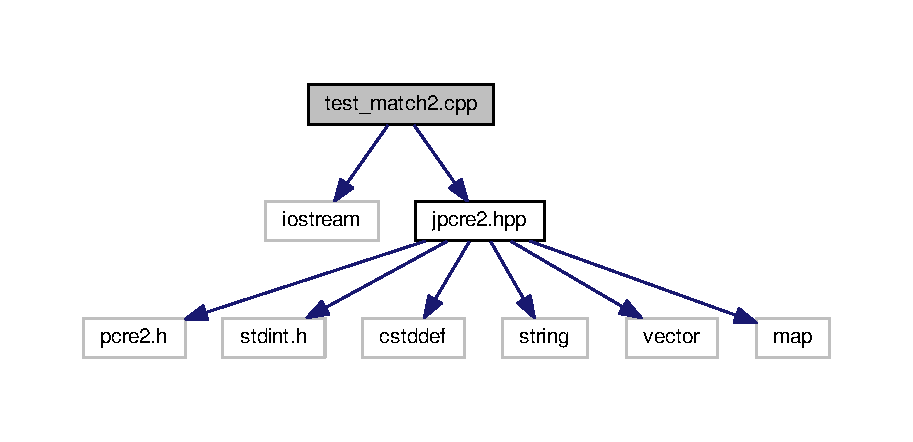
\includegraphics[width=350pt]{test__match2_8cpp__incl}
\end{center}
\end{figure}


\subsubsection{Detailed Description}
Contains an example to take subject string, pattern and modifier from user input and perform regex match using J\+P\+C\+R\+E2. 


\begin{DoxyCodeInclude}

\textcolor{preprocessor}{#include <iostream>}
\textcolor{preprocessor}{#include "\hyperlink{jpcre2_8hpp}{jpcre2.hpp}"}


\textcolor{preprocessor}{#define getLine(a) std::getline(std::cin,a,'\(\backslash\)n')}


\textcolor{keywordtype}{int} main()\{

    \hyperlink{namespacejpcre2_ac1cf752c8fbb0be78020be3b80e77ce3}{jpcre2::VecNum} vec\_num0;   \textcolor{comment}{//Vector to store numbered substring Map.}
    \hyperlink{namespacejpcre2_a2b121ae776ea5b2913839f418a7d856b}{jpcre2::VecNas} vec\_nas0;   \textcolor{comment}{//Vector to store named substring Map.}
    \hyperlink{namespacejpcre2_a88a7aaf84cad627d34c8152e726168eb}{jpcre2::VecNtN} vec\_nn0;    \textcolor{comment}{//Vector to store Named substring to Number Map.}
    
   
    std::string pat, mod, subject, ac\_mod;
    
    \textcolor{comment}{//create an object}
    \hyperlink{classjpcre2_1_1Regex}{jpcre2::Regex} re;

    std::cout<<\textcolor{stringliteral}{"Enter pattern: "};
    getLine(pat);
    
    \textcolor{keywordflow}{while}(\textcolor{keyword}{true})\{
        std::cout<<\textcolor{stringliteral}{"Enter compile modifiers (eijmnsuxADJSU): "};
        getLine(mod);
        
        \textcolor{comment}{//Compile pattern}
        re.\hyperlink{classjpcre2_1_1Regex_aad1d5ef1e87f762f68a587eec4022e69_aad1d5ef1e87f762f68a587eec4022e69}{compile}(pat, mod);
        
        \textcolor{comment}{//Check if the pattern was compiled successfully, continue the loop otherwise}
        \textcolor{keywordflow}{if}(!re)\{std::cerr<<re.\hyperlink{classjpcre2_1_1Regex_a8606fff8b192c94f58ca9e82aa048c61_a8606fff8b192c94f58ca9e82aa048c61}{getErrorMessage}()<<std::endl;\textcolor{keywordflow}{continue};\}
        \textcolor{keywordflow}{break};
    \}
    
    std::cout<<\textcolor{stringliteral}{"\(\backslash\)nPattern compiled with modifiers: "}<<re.\hyperlink{classjpcre2_1_1Regex_a0ac4e063f00128b96cd94c33609dc559_a0ac4e063f00128b96cd94c33609dc559}{getModifier}();

    \textcolor{keywordtype}{size\_t} matched = 0;
    
    re.\hyperlink{classjpcre2_1_1Regex_a519b0915bf1163c6ce6a4d674b30cfcd_a519b0915bf1163c6ce6a4d674b30cfcd}{initMatch}()                                \textcolor{comment}{//invoke the initMatch() function}
      .\hyperlink{classjpcre2_1_1RegexMatch_a2c7efe1ec2e13827f670db4ecedcd0a0_a2c7efe1ec2e13827f670db4ecedcd0a0}{setNumberedSubstringVector}(&vec\_num0)      \textcolor{comment}{//pointer to numbered substring
       vector}
      .\hyperlink{classjpcre2_1_1RegexMatch_ae495431f57cae54363331237ab21b56c_ae495431f57cae54363331237ab21b56c}{setNamedSubstringVector}(&vec\_nas0)         \textcolor{comment}{//pointer to named substring
       vector}
      .\hyperlink{classjpcre2_1_1RegexMatch_a04926e61d8b5f1d8bdf344efecd567d8_a04926e61d8b5f1d8bdf344efecd567d8}{setNameToNumberMapVector}(&vec\_nn0)         \textcolor{comment}{//pointer to name-to-number map
       vector}
      \textcolor{comment}{//.match()                                  //Let's do the match later}
      ;
        
        
    \textcolor{keywordflow}{for}(;;) \{ \textcolor{comment}{//forever loop}
        
        std::cout<<\textcolor{stringliteral}{"\(\backslash\)nEnter subject string (enter quit to quit): "}<<std::endl;
        getLine(subject);
        \textcolor{keywordflow}{if}(subject == \textcolor{stringliteral}{"quit"}) \textcolor{keywordflow}{break};
        
        std::cout<<\textcolor{stringliteral}{"\(\backslash\)nEnter action (matching) modifier (Ag): "}<<std::endl;
        getLine(ac\_mod);
        
        \textcolor{comment}{//Now let's do the match}
        matched = re.\hyperlink{classjpcre2_1_1Regex_abb007e99d7e2188ec80b741e7b40668f_abb007e99d7e2188ec80b741e7b40668f}{getMatchObject}()                           \textcolor{comment}{//returns a reference to the
       previously initialized match object}
                    .\hyperlink{classjpcre2_1_1RegexMatch_a635c652195deaa8ebb9e107c4f972aab_a635c652195deaa8ebb9e107c4f972aab}{setSubject}(subject)                      \textcolor{comment}{//subject}
                    .\hyperlink{classjpcre2_1_1RegexMatch_a08c2e481fe8b9c001e67733fb4e33972_a08c2e481fe8b9c001e67733fb4e33972}{addModifier}(ac\_mod)                        \textcolor{comment}{//add modifier}
                    .\hyperlink{classjpcre2_1_1RegexMatch_a5868aef3a146594ea1ebef34d122bb33_a5868aef3a146594ea1ebef34d122bb33}{match}();                                   \textcolor{comment}{//Now perform the match}
          
        \textcolor{comment}{//Now let's access the matched data}

        \textcolor{comment}{//Each of these vectors contains maps.}
        \textcolor{comment}{//Each element in the vector specifies a particular match}
        \textcolor{comment}{//First match is the vector element 0, second is at index 1 and so forth}
        \textcolor{comment}{//A map for a vector element, i.e for a match contains all of its substrings/capture groups}
        \textcolor{comment}{//The first element of the map is capture group 0 i.e total match}
        std::cout<<\textcolor{stringliteral}{"\(\backslash\)nTotal number of matches: "}<<matched<<std::endl;
        \textcolor{keywordflow}{if}(matched)\{
            \textcolor{keywordflow}{for}(\textcolor{keywordtype}{size\_t} i=0;i<vec\_num0.size();++i)\{
                
                
                std::cout<< \textcolor{stringliteral}{"\(\backslash\)n################## Match no: "}<<i+1<<\textcolor{stringliteral}{" ####################\(\backslash\)n"};
                
                
                
                \textcolor{comment}{//This vector contains maps with number as the key and the corresponding substring as the
       value}
                std::cout<<\textcolor{stringliteral}{"\(\backslash\)n-------------------------------------------------------------------------"};
                std::cout<< \textcolor{stringliteral}{"\(\backslash\)n--- Numbered Substrings (number: substring) for match "}<<i+1<<\textcolor{stringliteral}{" ---\(\backslash\)n"};
                \textcolor{keywordflow}{for}(jpcre2::MapNum::iterator ent=vec\_num0[i].begin();ent!=vec\_num0[i].end();++ent)\{
                    std::cout<<\textcolor{stringliteral}{"\(\backslash\)n\(\backslash\)t"}<<ent->first<<\textcolor{stringliteral}{": "}<<ent->second<<\textcolor{stringliteral}{"\(\backslash\)n"};
                \}
                
                
                
                \textcolor{comment}{//This vector contains maps with name as the key and the corresponding substring as the
       value}
                std::cout<<\textcolor{stringliteral}{"\(\backslash\)n-------------------------------------------------------------------------"};
                std::cout<< \textcolor{stringliteral}{"\(\backslash\)n--- Named Substrings (name: substring) for match "}<<i+1<<\textcolor{stringliteral}{" ---\(\backslash\)n"};
                \textcolor{keywordflow}{for}(jpcre2::MapNas::iterator ent=vec\_nas0[i].begin();ent!=vec\_nas0[i].end();++ent)\{
                    std::cout<<\textcolor{stringliteral}{"\(\backslash\)n\(\backslash\)t"}<<ent->first<<\textcolor{stringliteral}{": "}<<ent->second<<\textcolor{stringliteral}{"\(\backslash\)n"};
                \}
                
                
                
                \textcolor{comment}{//This vector contains maps with name as the key and number as the value}
                \textcolor{comment}{//i.e the number (of substring) can be accessed with the name for named substring.}
                std::cout<<\textcolor{stringliteral}{"\(\backslash\)n-------------------------------------------------------------------------"};
                std::cout<< \textcolor{stringliteral}{"\(\backslash\)n--- Name to number mapping (name: number/position) for match "}<<i+1<<\textcolor{stringliteral}{" ---\(\backslash\)n
      "};
                \textcolor{keywordflow}{for}(jpcre2::MapNtN::iterator ent=vec\_nn0[i].begin();ent!=vec\_nn0[i].end();++ent)\{
                    std::cout<<\textcolor{stringliteral}{"\(\backslash\)n\(\backslash\)t"}<<ent->first<<\textcolor{stringliteral}{": "}<<ent->second<<\textcolor{stringliteral}{"\(\backslash\)n"};
                \}
            \}
        \}
        \textcolor{keywordflow}{else} std::cout<<\textcolor{stringliteral}{"\(\backslash\)nNo match found\(\backslash\)n"};
    \}
    \textcolor{keywordflow}{return} 0;
\}
\end{DoxyCodeInclude}
 \begin{DoxyAuthor}{Author}
\href{https://github.com/neurobin}{\tt Md Jahidul Hamid} 
\end{DoxyAuthor}
